
\labtitle{\semester}{1}{Monday, August 31/Tuesday, September 1}

\section*{Problem 1: Unique Character Strings} 

\textit{Given a string of length $n$, determine whether it contains all unique characters - or, whether any characters are used more than once.}\\

\textit{Tips:} Guess the lower-bound! What is the limit on the fastest runtime algorithm that anyone can formulate for this problem?\\

\textbf{Naive Solution.} Iterate through each character $c$ in the string $s$. For each such $c$, iterate starting from the next character to the end of the string. If a duplicate character appears, return false. Otherwise, return true.\\

\begin{java}
    //naive solution
    boolean hasNoRepeats(String s) {
        for (int i = 0; i < s.length(); i++) {
            for (int j = i+1; j < s.length(); j++) {
                if (s.charAt(i) == s.charAt(j)) {
                    return false;
                }
            }
        }
        return true;
    }
\end{java}

\textit{Runtime:} Quadratic.\\

How might you guess that you could improve this runtime? Notice how this algorithm will repeat itself by examining the same parts of the string over and over again. Trying to avoid pointless repetition is a key to success.\\

\textbf{Alternate solution.} Suppose the string $s$ only contains characters from the English alphabet. Create a boolean array $B$ of size $26$, with all values initially false. Iterate through $s$ and examine each character in order. Suppose that at any particular point in the iteration WLOG you have the $i$th character in the alphabet. Check if $B[i]$ is true. If it is, return false. Otherwise, set it to true and continue. At the end of the iteration, return true.\\

\textit{Runtime:} Linear (in terms $n$). Space usage is constant.\\

\textit{Suggested improvements:} Use a bitstring of maximal size $\log m$ instead of an array. ($m$ is size of the alphabet.) Example solution in C shown on the next page, \textbf{for the 240 folk.} (It's ok if you don't understand. C is not covered in this course!)\\

\textbf{Alternate solution 2.} Iterate through each character of the string and add each to a set $S$. If $S$ already contains the character, return false. Otherwise, return true.\\

\textit{Runtime:} It depends! How is the set implemented? Is it a black box? If you don't know the runtime of set add/contains, you can't use this result.\\

\begin{code}{c}
    // pr0.c
    // Implementation of alternate solution 1.
    // READ IF CURIOUS. NOT COVERED IN COURSE MATERIAL.
    // Returns 1 if string has no repeat characters.
    // Otherwise, returns 0 if it finds any.
    // 
    // @param s - string of lowercase alphabetical chars

    int hasNoRepeats(char *s) {
        unsigned int b = 0;

        for (int i = 0; i < strlen(s); i++) {
            int offset = s[i] - 'a';

            if (1 & b >> offset) {  //Examine the ith bit.
                return 0;           //If set, duplicate found!
            }

            b |= (1 << offset);     //Mark bit as found.
        }

        return 1;
    }
\end{code}

\section*{Problem 2: Anagram Strings}

\textit{Given two strings, determine whether they are anagrams of each other.}

\begin{center}
    \texttt{TOMMARVOLORIDDLE} $\longleftrightarrow$ \texttt{IAMLORDVOLDEMORT}\\

    \textit{The above are anagrams of each other!\\ (Sorry if I spoiled book 2 of Harry Potter for you...)}
\end{center}

\textbf{Solution 1.} Suppose the two strings are $s_1$ and $s_2$ and we are allowed to modify them. Compare their lengths. If unequal, return false. Compare the strings. If they are equal, return true. Iterate through $s_1$. For each character $c$, try removing $c$ from $s_2$. If $c \notin s_2$, return false. When finished, if $s_2$ is not empty, return false. Return true otherwise.\\

\textit{Runtime: } Quadratic. At each iteration we search in $s_2$, doing $n + (n-1) + (n-2) + ... + 1 = \frac{n\cdot(n+1)}{2}$ total work in the worst case.\\

\textbf{Solution 2.} Sort both strings and compare them for equality.\\

\textit{Runtime: } It depends. There are variety of sorting algorithms out there, from the speedy quicksort to the \textit{infamous} bogosort! Using quicksort or any comparison based sort, the lower bound will be linear-logarithmic ($n \log n$). You'll learn more about this later in the course.\\

\textbf{Solution 3.} Suppose the two strings are $s_1$ and $s_2$ and that both have a fixed alphabet (English). Create two arrays, $A$ and $B$ and initialize their entries to $0$. Iterate through $s_1$. For each character $c$, if it is the $i$th letter in the alphabet, increment $A[i]$. Repeat for $s_2$, using $B$ instead. When finished, iterate through $A$ and $B$ at the same time,
comparing the values of the entries. If for any $i$, $A[i] \neq B[i]$, return false. Otherwise, return true when finished.\\

\textit{Runtime:} Linear, and constant space. Observe that the first loop runs $n$ times. The second loop runs a constant number of times, also doing a constant amount of work.\\

\textit{Suggested improvements:} To improve space usage, instead of having two arrays - create one. Each time a character shows up in $s_1$, increment by 1. Each time a character appears in $s_2$, decrement by 1. In the second loop, check for nonzero entries.\\

\begin{java}
    /**
     * Returns whether two strings are anagrams of each other.
     *
     * @param s1, s2 - the input strings. Assumed to contain
     *                 only letters of the English alphabet.
     */
    boolean areAnagrams(String s1, String s2) {
        if (s1.length() != s2.length()) {
            return false;
        }
        if (s1.equals(s2)) {
            return true;
        }

        int A[] = new int[26], B[] = new int[26];
        for (int i = 0; i < s1.length(); i++) { //Compute the histograms of $s_1$, $s_2$.
            A[s1.charAt(i) - 'a']++;
            B[s2.charAt(i) - 'a']++;
        }

        for (int i = 0; i < 26; i++) {          //Compare histograms.
            if (A[i] != B[i]) {
                return false;
            }
        }

        return true;
    }
\end{java}
\section*{Problem 3: Dutch National Flag}

\textit{Given $n$ balls of three colors - say red, white, and blue - arranged randomly in a line, sort them as quickly as possible into contiguous groups of red, white, and blue, with the groups in that order.}\\

\begin{figure}[h]
    \centering
    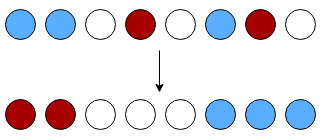
\includegraphics[width=\textwidth*3/8]{dutch_flag}
\end{figure}

\textit{How fast can generic sorts do this?}\\

Selection and insertion sort can do this in quadratic time. Not exactly the best choice.\\

Mergesort can solve this in linear-logarithmic time... but not in-place.\\

Quicksort can do the sort in average-case linear-logarithmic time and worst-case quadratic time, in-place.\\

\textbf{Linear-time algorithm.} Suppose the array $A$ is given as an input, which contains the initial ordering of the balls. Assume that red balls are represented as $0$'s, white $1$'s, and blue $2$'s. Create an array $B$ of size $3$, where the entries are initialized to $0$. Iterate through $A$. For each occurrence of a colored ball, increment the corresponding entry in $B$. When finished, iterate through $B$. For $i=0$, output $B[0]$ red balls - and so forth.\\

\begin{java}
    //
    int[] dutchNationalFlagSort(int[] A) {
        int B[] = new int[3];

        for (int b : A) {
            B[b]++;
        }

        int count = 0;
        for (int i = 0; i < B.length; i++) {
            for (int j = 0; j < B[i]; j++) {
                A[count++] = i;
            }
        }

        return A;
    }
\end{java}

The above is an implementation of \textbf{counting-sort}, which you'll learn later on (in CIS 320).

\section*{Problem 4: Row/Column-sorted Matrix Membership}
\textit{Given an $m$ by $n$ matrix of integers, where each row and each column of the matrix is sorted, determine whether an integer $k$ exists somewhere in the matrix.}
\begin{itemize}
    \item \textit{How could we do this if we didn't know the rows and columns were sorted?}
    
    \textbf{Solution 1.} If we can not presume anything about the structure of the matrix, we have no choice but to check each element manually! This of course leads to worst case $O(mn)$ time.

    \begin{java}
        public boolean containsK(int[][] A, int k) {
            for (int i = 0; i < A.length; i++)
                for (int j = 0; j < A[0].length; j++)
                    if (A[i][j] == k)
                        return true;
            return false;
        }
    \end{java}

    \item \textit{How does knowing the rows and columns are sorted let us do this faster?}

    If we know that the rows and columns are ordered (suppose in ascending order), this allows us to rule out certain parts of the matrix when searching.

    \textbf{Solution 2.} Compare $k$ to the top-right element of the matrix, $c$. If $k = c$, return true. If $k > c$, then we can rule out the top row because it is sorted and $c$ is its largest element. If $k < c$, then we can rule out the right column, since it is sorted and $c$ is the smallest element. Repeat until either $k$ is found or every row/column is eliminated without reaching the $k=c$ case. Return false.

    \item \textit{What is our optimal runtime?}

    The optimal runtime of the above algorithm is $O(m+n)$. At each iterative step, we eliminate either a row or a column and decreasing the overall problem size. Therefore, the worst case runtime is bounded by the total number of rows and columns.

    \begin{java}
        /**
         * Recursive implementation of linear-time search for
         * an element $k$ in $A$.
         * @param A - 2D array of integers, the input matrix
         * Guaranteed to have sorted rows and columns.
         * @param k - number to search for
         * @return whether or not $k$ is an element of $A$
         */
        public boolean containsK(int[][] A, int k) {
            return containsKHelper(A, 0, A[0].length-1, k);
        }

        /**
         * Recursive helper function for `containsK`.
         * Receives a 'submatrix' of the original that shrinks
         * as the algorithm eliminates rows/columns in it search.
         * @param A - 2D array of integers
         * @param minRow - the minimum row of the submatrix
         * @param maxCol - the maximum column of the submatrix
         * @param k - number to search for
         * @return whether or not $k$ is an element of $A$
         */
        public boolean containsKHelper(int[][] A, int minRow, int maxCol, int k) {
            // Base case.
            if (minRow >= A.length || maxCol < 0) {
                return false;
            }

            int c = A[minRow][maxCol];
            if (k == c)
                return true;
            else if (k > c)
                return containsK(A, minRow+1, maxCol, k);
            else
                return containsK(A, minRow, maxCol-1, k);
        }
    \end{java}
    
    \begin{java}
        /**
         * Iterative implementation of linear-time search
         * for an element $k$ in $A$.
         */
        public boolean containsK(int[][] A, int k) {
            int minRow = 0, maxCol = A[0].length-1;

            while (minRow < A.length && maxCol >= 0) {
                int c = A[minRow][maxCol];
                if (k == c)
                    return true;
                else if (k > c)
                    minRow++;
                else
                    maxCol--;
            }
            return false;
        }
    \end{java}

\end{itemize}
    
